% ***************************************************
% FORMATO.
% ***************************************************
\documentclass[a4paper,12pt]{article}
% Input encoding.
% Idioma.
\usepackage[spanish, es-tabla]{babel}
\usepackage[utf8]{inputenc}
% Ver pagina 92 de "The not so short introduction to Latex" por Tobias Oetiker
% para entender que hacen estos paquetes.
\usepackage{lmodern}
\usepackage[T1]{fontenc}
\usepackage{textcomp}
% Paquete para utilizar el font Times Roman de Adobe por defecto.
\usepackage{mathptmx}
 
%Manejo de márgenes
%Agrega 2cm al ancho por defecto (usado junto con hoffset, no se pierde el centrado)
\addtolength{\textwidth}{2cm}
%Quita 1cm al margen, pero mantiene la relación repecto de cada margen
\addtolength{\hoffset}{-1cm}
\addtolength{\textheight}{2cm}
\addtolength{\voffset}{-1cm}
\setlength{\headheight}{14pt}

% Paquete para manejo de headers y footers.
\usepackage{fancyhdr}
\usepackage{lastpage}
% Determinación del estilo de página (encabezado y pie). Debe ir luego del bloque de manejo de margenes para que
% no haya problemas de dimensiones. Por ejemplo, que el texto quede mas ancho que el encabezado o pie.
\pagestyle{fancy}
% Se borra el header y footer por defecto.
\fancyhf{}
\lhead{\small TP1 [2C2018]}
\chead{}
\rhead{\small [66.20] Organización de Computadoras}
\rfoot{}
\cfoot{Página {\thepage} de \pageref{LastPage}}
\lfoot{}

% Paquete para manejo de textos en varbatim en varios lugares del documento, por ejemplo en los headers.
\usepackage{fancyvrb}
% Paquete para manejo de boxes de manera mas flexible.
\usepackage{fancybox}

% Para no mostrar el numero de pagina, usar las siguientes dos lineas:
%\thispagestyle{empty}
%\setcounter{savepage}{\thepage}

% Paquete para hacer subrayados, poner textos en color y resaltar texto en color.
% Lo bueno de este paquete es que no tira errores de fullbox como cuando se usa \colorbox{declared-color}{text}.
% El unico problema es que no soporta acentos desde el teclado (tira un error de UTF8). Hay que incluirlos usando \'.
\usepackage{soul}
% Configura el paquete @SOUL para que el resaltado de texto sea rojo. La sintaxis es \hl{text}.
\sethlcolor{red}

% Paquete que deja sangria luego de comenzada una seccion nueva.
%\usepackage{indentfirst}

% Se define una macro para poner double quotes de manera simple. El uso es \quotes{Hello World!}.
\newcommand{\quotes}[1]{``#1''}

% ***************************************************
% MATEMATICA.
% ***************************************************
\usepackage{amsmath}
	% Formato de numeracion de ecuaciones por seccion. Ej. seccion x, ecuacion y: (x.y)
	\numberwithin{equation}{section}
	\numberwithin{figure}{section}
	
% Simbolos matematicos. Por ej. la 'R' de reales, etc...
\usepackage{amssymb}
\usepackage{amsfonts}

\usepackage{mathtools}

% Paquete para arrays de ecuaciones.
\usepackage[retainorgcmds]{IEEEtrantools}
% Unidad imaginaria.
\newcommand{\iu}{{j\mkern1mu}}
% Contador de uso generico.
\newcounter{hipotesis_ct}
\setcounter{hipotesis_ct}{1}

% Operador 'derivada'.
\makeatletter
\providecommand*{\diff}%
{\@ifnextchar^{\DIfF}{\DIfF^{}}}
\def\DIfF^#1{%
	\mathop{\mathrm{\mathstrut d}}%
	\nolimits^{#1}\gobblespace}
\def\gobblespace{%
	\futurelet\diffarg\opspace}
\def\opspace{%
	\let\DiffSpace\!%
	\ifx\diffarg(%
	\let\DiffSpace\relax
	\else
	\ifx\diffarg[%
	\let\DiffSpace\relax
	\else
	\ifx\diffarg\{%
	\let\DiffSpace\relax
	\fi\fi\fi\DiffSpace}

% Uso:
% \pderiv[n]{A}{B}
\providecommand*{\deriv}[3][]{%
	\frac{\diff^{#1}#2}{\diff #3^{#1}}}
\providecommand*{\pderiv}[3][]{%
	\frac{\partial^{#1}#2}%
	{\partial #3^{#1}}}

% Operadores 'valor absoluto' y 'norma'.
% Uso: \abs{123} \norm{123} \abs*{123} \norm*{123}
\DeclarePairedDelimiter\abs{\lvert}{\rvert}%
\DeclarePairedDelimiter\norm{\lVert}{\rVert}%
% Swap the definition of \abs* and \norm*, so that \abs
% and \norm resizes the size of the brackets, and the 
% starred version does not.
\makeatletter
\let\oldabs\abs
\def\abs{\@ifstar{\oldabs}{\oldabs*}}
%
\let\oldnorm\norm
\def\norm{\@ifstar{\oldnorm}{\oldnorm*}}
\makeatother

% Operadores para escribir vectores en negrita directamente.
% Ej:  $\vecbf{v} = 5\vechat{k}$ 
\newcommand{\vecbf}[1]{\mathbf{#1}}
% Operador para escribir en negrita todo lo que tenga hat.
\newcommand{\vechat}[1]{\hat{\mathbf{#1}}}

% ***************************************************
% CODIGO FUENTE.
% ***************************************************
% Paquetes para pseudocodigo.	
\usepackage{lgrind}
\usepackage{algorithm}
\usepackage{algpseudocode}
\makeatletter
\renewcommand{\ALG@name}{Algoritmo}
\renewcommand{\listalgorithmname}{Lista de \ALG@name s}
\algrenewcommand\algorithmicensure{\textbf{Salida:}}
\algrenewcommand\algorithmicrequire{\textbf{Entrada:}}
\algnewcommand{\LineComment}[1]{\State \(\triangleright\) #1}
\makeatother

% Paquete para incluir codigo de MatLab.
\usepackage[numbered,framed]{matlab-prettifier}
% Paquete para control de colores. Ya lo carga 'matlab-prettifier'.
\PassOptionsToPackage{usenames,dvipsnames}{xcolor}

% Fuente: http://en.wikibooks.org/wiki/LaTeX/Colors
\definecolor{Apricot}{RGB}{253,199,130}
\definecolor{Aquamarine}{RGB}{0,181,202}
\definecolor{Bittersweet}{RGB}{192,79,23}
\definecolor{Black}{RGB}{0,0,0}
\definecolor{Blue}{RGB}{0,0,255}
\definecolor{BlueGreen}{RGB}{0,179,184}
\definecolor{BlueViolet}{RGB}{71,57,146}
\definecolor{BrickRed}{RGB}{182,50,28}
\definecolor{Brown}{RGB}{121,37,0}
\definecolor{BurntOrange}{RGB}{247,146,29}
\definecolor{CadetBlue}{RGB}{116,114,154}
\definecolor{CarnationPink}{RGB}{242,130,180}
\definecolor{Cerulean}{RGB}{0,162,227}
\definecolor{CornflowerBlue}{RGB}{65,176,228}
\definecolor{Cyan}{RGB}{0,174,239}
\definecolor{Dandelion}{RGB}{253,188,66}
\definecolor{DarkOrchid}{RGB}{164,83,138}
\definecolor{Emerald}{RGB}{0,169,157}
\definecolor{ForestGreen}{RGB}{0,155,85}
\definecolor{Fuchsia}{RGB}{140,54,140}
\definecolor{Goldenrod}{RGB}{255,223,66}
\definecolor{Gray}{RGB}{148,150,152}
\definecolor{Green}{RGB}{0,166,79}
\definecolor{GreenYellow}{RGB}{223,230,116}
\definecolor{JungleGreen}{RGB}{0,169,154}
\definecolor{Lavender}{RGB}{244,158,196}
\definecolor{LimeGreen}{RGB}{141,199,62}
\definecolor{Magenta}{RGB}{236,0,140}
\definecolor{Mahogany}{RGB}{169,52,31}
\definecolor{Maroon}{RGB}{175,50,53}
\definecolor{Melon}{RGB}{248,158,123}
\definecolor{MidnightBlue}{RGB}{0,103,149}
\definecolor{Mulberry}{RGB}{169,60,147}
\definecolor{NavyBlue}{RGB}{0,103,149}
\definecolor{OliveGreen}{RGB}{60,128,49}
\definecolor{Orange}{RGB}{245,129,55}
\definecolor{OrangeRed}{RGB}{237,19,90}
\definecolor{Orchid}{RGB}{175,114,176}
\definecolor{Peach}{RGB}{247,150,90}
\definecolor{Periwinkle}{RGB}{121,119,184}
\definecolor{PineGreen}{RGB}{0,139,114}
\definecolor{Plum}{RGB}{146,38,143}
\definecolor{ProcessBlue}{RGB}{0,176,240}
\definecolor{Purple}{RGB}{153,71,155}
\definecolor{RawSienna}{RGB}{151,64,6}
\definecolor{Red}{RGB}{237,27,35}
\definecolor{RedOrange}{RGB}{242,96,70}
\definecolor{RedViolet}{RGB}{161,36,107}
\definecolor{Rhodamine}{RGB}{239,85,159}
\definecolor{RoyalBlue}{RGB}{0,113,188}
\definecolor{RoyalPurple}{RGB}{97,63,153}
\definecolor{RubineRed}{RGB}{237,1,125}
\definecolor{Salmon}{RGB}{246,146,137}
\definecolor{SeaGreen}{RGB}{63,188,157}
\definecolor{Sepia}{RGB}{103,24,0}
\definecolor{SkyBlue}{RGB}{70,197,221}
\definecolor{SpringGreen}{RGB}{198,220,103}
\definecolor{Tan}{RGB}{218,157,118}
\definecolor{TealBlue}{RGB}{0,174,179}
\definecolor{Thistle}{RGB}{216,131,183}
\definecolor{Turquoise}{RGB}{0,180,206}
\definecolor{Violet}{RGB}{88,66,155}
\definecolor{VioletRed}{RGB}{239,88,160}
\definecolor{White}{RGB}{255,255,255}
\definecolor{WildStrawberry}{RGB}{238,41,103}
\definecolor{Yellow}{RGB}{255,242,0}
\definecolor{YellowGreen}{RGB}{152,204,112}
\definecolor{YellowOrange}{RGB}{250,162,26}


\lstdefinestyle{StyleMake}{%
	linewidth=\textwidth,%		Define el ancho máximo de una linea de código
	xleftmargin=2.5pt,%				Margen izquierdo
	xrightmargin=2.5pt,%				Margen derecho
	breaklines=true,%				Que corte lineas largas
	numbers=left,%			Que haya números a la izquierda (número de linea)
	numberstyle=\scriptsize,%		Formato de los números de linea
	stepnumber=1,%					Que avancen de a 1 (ver todos los números)
	numbersep=10pt,%					La separación de los números del código
	tabsize=4,showtabs=false,%		Los TABS son 4 espacios, y no se ven
	extendedchars=true,%			Se permiten caracteres extendidos
	basicstyle=\ttfamily\small,%	Estilo básico de la tipografía del código
	commentstyle=\color{Blue},%		Color de los comentarios
	showstringspaces=false,%		Los espacios no se ven de forma especial
	stringstyle=\color{BrickRed},%	Estilo de las cadenas
	keywordstyle=\color{ForestGreen},%	Estilo de las palabras reservadas
	morekeywords=[1]{g++,-Wall,-pedantic},%	Definición de más palabras reservadas
	deletekeywords={rm,-rf,*.o},%
	keywords=[2]{rm,-rf,*.o},%
	keywordstyle=[2]{\color{BurntOrange}},%	2do grupo de palabras reservadas
	directives={CC,CFLAGS,OUTPUT},%
	directivestyle=\color{NavyBlue},%	Estilo de directivas
	keywords=[3]{CC,CFLAGS,OUTPUT},%
	keywordstyle=[3]{\color{MidnightBlue}},%3er grupo de palabras reservadas
	morecomment=[s][\color{Blue}]{/*}{*/}%	Definición de estilo de comentario
}

\lstdefinestyle{StyleC}{%
	linewidth=\textwidth,%		Define el ancho máximo de una linea de código
	xleftmargin=2.5pt,%				Margen izquierdo
	xrightmargin=2.5pt,%				Margen derecho
	breaklines=true,%				Que corte lineas largas
	numbers=left,%			Que haya números a la izquierda (número de linea)
	numberstyle=\scriptsize,%		Formato de los números de linea
	stepnumber=1,%					Que avancen de a 1 (ver todos los números)
	numbersep=10pt,%					La separación de los números del código
	tabsize=4,showtabs=false,%		Los TABS son 4 espacios, y no se ven
	extendedchars=true,%			Se permiten caracteres extendidos
	basicstyle=\ttfamily\small,%	Estilo básico de la tipografía del código
	commentstyle=\color{Blue},%		Color de los comentarios
	showstringspaces=false,%		Los espacios no se ven de forma especial
	stringstyle=\color{BrickRed},%	Estilo de las cadenas
	keywordstyle=\color{ForestGreen},%	Estilo de las palabras reservadas
	morekeywords=[1]{size_t,ssize_t},%	Definición de más palabras reservadas
	deletekeywords={typedef,enum,do,while,if,else,for,case,default,switch,break,continue},%
	keywords=[2]{typedef,enum,do,while,if,else,for,case,default,switch,break,continue,EXIT_SUCCESS,EXIT_FAILURE},%
	keywordstyle=[2]{\color{BurntOrange}},%	2do grupo de palabras reservadas
	directives={define,undef,include,if,else,ifndef,ifdef,elif,endif},%
	directivestyle=\color{NavyBlue},%		Estilo de directivas
	keywords=[3]{define,undef,include,if,else,ifndef,ifdef,elif,endif},%
	keywordstyle=[3]{\color{MidnightBlue}},%3er grupo de palabras reservadas
	morecomment=[s][\color{Blue}]{/*}{*/}%	Definición de estilo de comentario
}

\lstnewenvironment{terminalblock}{%
	\lstset{style=StyleC}}{}

\lstset{
	literate={ö}{{\"o}}1
	{ä}{{\"a}}1
	{ü}{{\"u}}1
	{á}{{\'a}}1
	{Á}{{\'A}}1
	{é}{{\'e}}1
	{É}{{\'E}}1
	{í}{{\'i}}1
	{Í}{{\'I}}1
	{ñ}{{\~n}}1
	{ó}{{\'o}}1
	{Ó}{{\'O}}1
	{ú}{{\'u}}1
	{Ú}{{\'U}}1
}

\definecolor{listinggray}{gray}{0.9}
\definecolor{lbcolor}{rgb}{0.9,0.9,0.9}
% http://tex.stackexchange.com/questions/44282/multiline-comment
\newcommand{\comment}[1]{}

\lstset{
	backgroundcolor=\color{lbcolor},
	tabsize=4,    
	language=[GNU]C++,
	basicstyle=\scriptsize,
	upquote=true,
	aboveskip={1.5\baselineskip},
	columns=fixed,
	showstringspaces=false,
	extendedchars=false,
	breaklines=true,
	prebreak = \raisebox{0ex}[0ex][0ex]{\ensuremath{\hookleftarrow}},
	frame=single,
	numbers=left,
	showtabs=false,
	showspaces=false,
	showstringspaces=false,
	identifierstyle=\ttfamily,
	keywordstyle=\color[rgb]{0,0,1},
	commentstyle=\color[rgb]{0.026,0.112,0.095},
	stringstyle=\color[rgb]{0.627,0.126,0.941},
	numberstyle=\color[rgb]{0.205, 0.142, 0.73},
}

\lstset{
	backgroundcolor=\color{lbcolor},
	tabsize=4,
	language=C++,
	captionpos=b,
	tabsize=3,
	frame=lines,
	numbers=left,
	numberstyle=\tiny,
	numbersep=5pt,
	breaklines=true,
	showstringspaces=false,
	basicstyle=\footnotesize,
	keywordstyle=\color[rgb]{0,0,1},
	commentstyle=\color[rgb]{0.026,0.112,0.095},
	stringstyle=\color{red},
}
% ***************************************************
% GRAFICOS.
% ***************************************************
	% Paquete para mejorar la interfaz con objetos flotantes, como los graficos.
	\usepackage{float}
	\usepackage{graphicx}
	% Paquetes para tener mayor flexibilidad cuando se utilizan titulos para figuras, etc...
	\usepackage{caption}
	\usepackage{subcaption}
	\usepackage{epstopdf}

% ***************************************************
% TABLAS.
% ***************************************************
% Paquetes para manejo de tablas.
\usepackage{booktabs}
\usepackage{multirow}

% ***************************************************
% MISC.
% ***************************************************
%\usepackage{draftwatermark}
%\SetWatermarkLightness{0.95}
%\SetWatermarkScale{0.8}
%\SetWatermarkText{BORRADOR}

% This pack­age sim­pli­fies the in­clu­sion of ex­ter­nal multi-page PDF doc­u­ments in LaTeX doc­u­ments. 
\usepackage{pdfpages}
\setboolean{@twoside}{false}

% Unidades del SI
\usepackage{siunitx}

% Adds bibliography section to the TOC.
\usepackage[nottoc,notlot,notlof]{tocbibind}

% ***************************************************
% TIKZ.
% ***************************************************
%\usepackage{tikz}
%\usetikzlibrary{calc,fadings,decorations.pathreplacing}
%%% helper macros
%\newcommand\pgfmathsinandcos[3]{%
%	\pgfmathsetmacro#1{sin(#3)}%
%	\pgfmathsetmacro#2{cos(#3)}%
%}
%\newcommand\LongitudePlane[3][current plane]{%
%	\pgfmathsinandcos\sinEl\cosEl{#2} % elevation
%	\pgfmathsinandcos\sint\cost{#3} % azimuth
%	\tikzset{#1/.estyle={cm={\cost,\sint*\sinEl,0,\cosEl,(0,0)}}}
%}
%\newcommand\LatitudePlane[3][current plane]{%
%	\pgfmathsinandcos\sinEl\cosEl{#2} % elevation
%	\pgfmathsinandcos\sint\cost{#3} % latitude
%	\pgfmathsetmacro\yshift{\cosEl*\sint}
%	\tikzset{#1/.estyle={cm={\cost,0,0,\cost*\sinEl,(0,\yshift)}}} %
%}
%\newcommand\DrawLongitudeCircle[2][1]{
%	\LongitudePlane{\angEl}{#2}
%	\tikzset{current plane/.prefix style={scale=#1}}
%	% angle of "visibility"
%	\pgfmathsetmacro\angVis{atan(sin(#2)*cos(\angEl)/sin(\angEl))} %
%	\draw[current plane] (\angVis:1) arc (\angVis:\angVis+180:1);
%	\draw[current plane,dashed] (\angVis-180:1) arc (\angVis-180:\angVis:1);
%}
%\newcommand\DrawLatitudeCircle[2][1]{
%	\LatitudePlane{\angEl}{#2}
%	\tikzset{current plane/.prefix style={scale=#1}}
%	\pgfmathsetmacro\sinVis{sin(#2)/cos(#2)*sin(\angEl)/cos(\angEl)}
%	% angle of "visibility"
%	\pgfmathsetmacro\angVis{asin(min(1,max(\sinVis,-1)))}
%	\draw[current plane] (\angVis:1) arc (\angVis:-\angVis-180:1);
%	\draw[current plane,dashed] (180-\angVis:1) arc (180-\angVis:\angVis:1);
%}
%
%%% document-wide tikz options and styles
%\tikzset{%
%	>=latex, % option for nice arrows
%	inner sep=0pt,%
%	outer sep=2pt,%
%	mark coordinate/.style={inner sep=0pt,outer sep=0pt,minimum size=3pt,
%		fill=black,circle}%
%}

% ***************************************************
% HIPERTEXTO.
% ***************************************************
% Paquete para utilizar hipertexto (tiene que ser siempre el ultimo paquete que se carga).
% Todos los links, referencias, etc...pasan a ser hipertextos.
% Setup del paquete de hipertexto.
\usepackage[pdftex,breaklinks]{hyperref}
	\hypersetup{a4paper,
				% Muestra el titulo en el maro superior de la ventana del visor de pdf
				pdfdisplaydoctitle=true,
				% Al encender esta funcion, ya nohay recuadros feos alrededor de los links 	
				colorlinks=true,
				% Color cuando se escribe una URL.   
				urlcolor = black,
				%Para que el link a nuevos pdf, no se abran en la misma ventana 		
				pdfnewwindow=true,
				% Color para links internos
				linkcolor=black,
				% Color para links a Bibliografia
				citecolor=black,
				% Color para links a archivos
       			filecolor=black,
				pdftitle={66.20 - TP1 - 2C2018},
				pdfauthor={AHV}
			}

% ***************************************************			
% GLOSARIO.
% ***************************************************
% Glosario. Debe cargarse después del paquete "hyperref", como excepción.
%\include{./misc/glossary}

% ***************************************************			
% ALGUNOS TEMPLATES DE CODIGO UTIL.
% ***************************************************

% *********************************************************************************
% Si incluyo figuras de MatLab, no conviene que se guarden maximizadas.
%\begin{figure}[!ht]
%	\centering
%	\includegraphics[scale=0.9]{includes/ex1_N5.eps}
%	\caption{Submuestreo con $N=5$ con $M=3$ y $M=6$}
%	\label{ex1_N5}
%\end{figure}
% *********************************************************************************
%\begin{figure}[H]
%	\centering
%	\begin{subfigure}[c]{0.3\textwidth}
%		\includegraphics[scale=0.06]{./includes/cover/Logo_UBA.eps}
%	\end{subfigure}
%	\begin{subfigure}[c]{0.3\textwidth}
%		\includegraphics[scale=0.5]{./includes/cover/Logo_FIUBA.eps}
%	\end{subfigure}
%\end{figure}
% *********************************************************************************
%\begin{IEEEeqnarray}{rCl}
%\IEEEyesnumber\label{ec_ex1_relaciones} \IEEEyessubnumber*
%x\left( n \right)  \  &=& \, x\left( n + k \, N \right) \label{ec_ex1_x}\\
%y\left( n \right)  \, &=& \, y\left( n + l \, L \right) \label{ec_ex1_y}\\
%y\left( n \right)  \, &=& \, x\left( M \, n \right) \label{ec_ex1_downsampling}
%\end{IEEEeqnarray}
%\begin{IEEEeqnarray}{CC}
%	\IEEEyesnumber\label{eq:both} \IEEEyessubnumber*
%	bla bla & blub blub \label{eq:sub1}\\
%	bla bla & bla bla  \label{eq:sub2}
%\end{IEEEeqnarray}
%where the set of equations \eqref{eq:sub1} and \eqref{eq:sub2}
%is referred to as \eqref{eq:both}.
%\begin{align}
%N_{x,sk} &= k_{sk}\left(\frac{t_{sk}}{b_{sk}}\right)^{2}\bar{Et}\nonumber\\
%N_{x,st} &= k_{st}\left(\frac{t_{st}}{b_{st}}\right)^{2}\bar{Et}
%\end{align}
% *********************************************************************************
%\begin{equation}
%\begin{cases}
%H\left( z \right) &= \sum_{l=0}^{M-1} \, z^{-l} \, E_l\left( z^M \right) \\
%E_l\left( z \right) &= \sum_{n=-\infty}^{+\infty} \, e_l \left( n \right) \, z^{-n} \\
%e_l\left( n \right) &= h\left(n\,M + l\right) \quad 0 \leq l \leq M-1
%\end{cases}
%\end{equation}
% *********************************************************************************
%\begin{equation}
%\mathbf{R}_x\left(\phi\right) = 
%\begin{bmatrix}
%1 & 0 & 0 \\
%0 & \cos \left(\phi\right) & \sin \left(\phi\right) \\
%0 & -\sin \left(\phi\right) & \cos \left(\phi\right) \\
%\end{bmatrix}
%\end{equation}
% *********************************************************************************
%\begin{algorithm}[!ht]
%\caption{Pseudocódigo del algoritmo euclídeo extendido}\label{alg_euc_ex}
%\begin{algorithmic}[1]
%\Require $H_0\left(z\right)$ y $H_1\left(z\right)$ coprimos
%\Ensure  $F_0\left(z\right)$ y $F_1\left(z\right)$ tales que $H_0\left(z\right)\cdot F_0\left(z\right)+H_1\left(z\right)\cdot F_1\left(z\right) = c$, con $c\neq0$. Además, $gr\left(F_0\right) < gr\left(H_1\right) - gr\left(g\right)$ y $gr\left(F_1\right) < gr\left(H_0\right) - gr\left(g\right)$.
%\Statex
%\Procedure{extEuclidean}{}
%\Statex
%\State Inicialización.
%\Statex
%\State $r_0=H_0 \quad r_1=H_1 \quad s_0=1 \quad s_1=0 \quad t_0=0 \quad t_1=1 \quad i=1$
%\Statex
%\While {$r_i\neq0 \quad\wedge\quad gr\left(r_{i+1}\right)\geqslant gr\left(r_i\right)$:}
%\Statex
%\State $q \leftarrow$ Cociente de $r_{i-1}/r_i$
%\Statex
%\State $r_{i+1} = r_{i-1} - q\,r_i$
%\Statex
%\State $s_{i+1} = s_{i-1} - q\,s_i$
%\Statex
%\State $t_{i+1} = t_{i-1} - q\,t_i$
%\Statex
%\State $i = i+1$
%\EndWhile
%\Statex
%\State $F_0\left(z\right) = s_{i-1} \quad F_1\left(z\right)=t_{i-1} \quad g=r_{i-1}$
%\EndProcedure
%\end{algorithmic}
%\end{algorithm}
% *********************************************************************************
%\begin{table}
%	\caption{A badly formatted table}
%	\centering
%	\label{table:bad_table}
%	\begin{tabular}{|l|c|c|c|c|}
%		\hline 
%		& \multicolumn{2}{c}{Species I} & \multicolumn{2}{c|}{Species II} \\ 
%		\hline
%		Dental measurement  & mean & SD  & mean & SD  \\ \hline 
%		\hline
%		I1MD & 6.23 & 0.91 & 5.2  & 0.7  \\
%		\hline 
%		I1LL & 7.48 & 0.56 & 8.7  & 0.71 \\
%		\hline 
%		I2MD & 3.99 & 0.63 & 4.22 & 0.54 \\
%		\hline 
%		I2LL & 6.81 & 0.02 & 6.66 & 0.01 \\
%		\hline 
%		CMD & 13.47 & 0.09 & 10.55 & 0.05 \\
%		\hline 
%		CBL & 11.88 & 0.05 & 13.11 & 0.04\\ 
%		\hline 
%	\end{tabular}
%\end{table}
% *********************************************************************************
%\begin{table}
%	\caption{A nice looking table}
%	\centering
%	\label{table:nice_table}
%	\begin{tabular}{l c c c c}
%		\hline 
%		\multirow{2}{*}{Dental measurement} & \multicolumn{2}{c}{Species I} & \multicolumn{2}{c}{Species II} \\ 
%		\cline{2-5}
%		& mean & SD  & mean & SD  \\ 
%		\hline
%		I1MD & 6.23 & 0.91 & 5.2  & 0.7  \\
%		
%		I1LL & 7.48 & 0.56 & 8.7  & 0.71 \\
%		
%		I2MD & 3.99 & 0.63 & 4.22 & 0.54 \\
%		
%		I2LL & 6.81 & 0.02 & 6.66 & 0.01 \\
%		
%		CMD & 13.47 & 0.09 & 10.55 & 0.05 \\
%		
%		CBL & 11.88 & 0.05 & 13.11 & 0.04\\ 
%		\hline 
%	\end{tabular}
%\end{table}
% *********************************************************************************
%\begin{table}
%	\caption{Even better looking table using booktabs}
%	\centering
%	\label{table:good_table}
%	\begin{tabular}{l c c c c}
%		\toprule
%		\multirow{2}{*}{Dental measurement} & \multicolumn{2}{c}{Species I} & \multicolumn{2}{c}{Species II} \\ 
%		\cmidrule{2-5}
%		& mean & SD  & mean & SD  \\ 
%		\midrule
%		I1MD & 6.23 & 0.91 & 5.2  & 0.7  \\
%		
%		I1LL & 7.48 & 0.56 & 8.7  & 0.71 \\
%		
%		I2MD & 3.99 & 0.63 & 4.22 & 0.54 \\
%		
%		I2LL & 6.81 & 0.02 & 6.66 & 0.01 \\
%		
%		CMD & 13.47 & 0.09 & 10.55 & 0.05 \\
%		
%		CBL & 11.88 & 0.05 & 13.11 & 0.04\\ 
%		\bottomrule
%	\end{tabular}
%\end{table}
% *********************************************************************************
%\begin{table}[htbp]
%	\centering
%	\caption{Primeros 40 coeficientes correspondientes a la Teoría de Nutación IAU-1980.}
%	\begin{tabular}{cccccccccc}
%		\toprule
%		\multicolumn{1}{c}{Coeficiente} & \multicolumn{1}{c}{$p_l$} & \multicolumn{1}{c}{$p_l'$} & \multicolumn{1}{c}{$p_F$} & \multicolumn{1}{c}{$p_D$} & \multicolumn{1}{c}{$p_\Omega$} & \multicolumn{1}{c}{$\Delta \hat{\psi} \left[0.001''\right]$} & \multicolumn{1}{c}{$\Delta \hat{\psi}_T\left[0.001''\right]$} & \multicolumn{1}{c}{$\Delta \hat{\varepsilon}\left[0.001''\right]$} & \multicolumn{1}{c}{$\Delta \hat{\varepsilon}_T\left[0.001''\right]$} \\
%		\midrule
%		1     & 0     & 0     & 0     & 0     & 1     & -1719960 & -1742 & 920250 & 89 \\
%		2     & 0     & 0     & 0     & 0     & 2     & 20620 & 2     & -8950 & 5 \\
%		3     & -2    & 0     & 2     & 0     & 1     & 460   & 0     & -240  & 0 \\
%		4     & 2     & 0     & -2    & 0     & 0     & 110   & 0     & 0     & 0 \\
%		5     & -2    & 0     & 2     & 0     & 2     & -30   & 0     & 10    & 0 \\
%		6     & 1     & -1    & 0     & -1    & 0     & -30   & 0     & 0     & 0 \\
%		7     & 0     & -2    & 2     & -2    & 1     & -20   & 0     & 10    & 0 \\
%		8     & 2     & 0     & -2    & 0     & 1     & 10    & 0     & 0     & 0 \\
%		9     & 0     & 0     & 2     & -2    & 2     & -131870 & -16   & 57360 & -31 \\
%		10    & 0     & 1     & 0     & 0     & 0     & 14260 & -34   & 540   & -1 \\
%		11    & 0     & 1     & 2     & -2    & 2     & -5170 & 12    & 2240  & -6 \\
%		12    & 0     & -1    & 2     & -2    & 2     & 2170  & -5    & -950  & 3 \\
%		13    & 0     & 0     & 2     & -2    & 1     & 1290  & 1     & -700  & 0 \\
%		14    & 2     & 0     & 0     & -2    & 0     & 480   & 0     & 10    & 0 \\
%		15    & 0     & 0     & 2     & -2    & 0     & -220  & 0     & 0     & 0 \\
%		16    & 0     & 2     & 0     & 0     & 0     & 170   & -1    & 0     & 0 \\
%		17    & 0     & 1     & 0     & 0     & 1     & -150  & 0     & 90    & 0 \\
%		18    & 0     & 2     & 2     & -2    & 2     & -160  & 1     & 70    & 0 \\
%		19    & 0     & -1    & 0     & 0     & 1     & -120  & 0     & 60    & 0 \\
%		20    & -2    & 0     & 0     & 2     & 1     & -60   & 0     & 30    & 0 \\
%		21    & 0     & -1    & 2     & -2    & 1     & -50   & 0     & 30    & 0 \\
%		22    & 2     & 0     & 0     & -2    & 1     & 40    & 0     & -20   & 0 \\
%		23    & 0     & 1     & 2     & -2    & 1     & 40    & 0     & -20   & 0 \\
%		24    & 1     & 0     & 0     & -1    & 0     & -40   & 0     & 0     & 0 \\
%		25    & 2     & 1     & 0     & -2    & 0     & 10    & 0     & 0     & 0 \\
%		26    & 0     & 0     & -2    & 2     & 1     & 10    & 0     & 0     & 0 \\
%		27    & 0     & 1     & -2    & 2     & 0     & -10   & 0     & 0     & 0 \\
%		28    & 0     & 1     & 0     & 0     & 2     & 10    & 0     & 0     & 0 \\
%		29    & -1    & 0     & 0     & 1     & 1     & 10    & 0     & 0     & 0 \\
%		30    & 0     & 1     & 2     & -2    & 0     & -10   & 0     & 0     & 0 \\
%		31    & 0     & 0     & 2     & 0     & 2     & -22740 & -2    & 9770  & -5 \\
%		32    & 1     & 0     & 0     & 0     & 0     & 7120  & 1     & -70   & 0 \\
%		33    & 0     & 0     & 2     & 0     & 1     & -3860 & -4    & 2000  & 0 \\
%		34    & 1     & 0     & 2     & 0     & 2     & -3010 & 0     & 1290  & -1 \\
%		35    & 1     & 0     & 0     & -2    & 0     & -1580 & 0     & -10   & 0 \\
%		36    & -1    & 0     & 2     & 0     & 2     & 1230  & 0     & -530  & 0 \\
%		37    & 0     & 0     & 0     & 2     & 0     & 630   & 0     & -20   & 0 \\
%		38    & 1     & 0     & 0     & 0     & 1     & 630   & 1     & -330  & 0 \\
%		39    & -1    & 0     & 0     & 0     & 1     & -580  & -1    & 320   & 0 \\
%		40    & -1    & 0     & 2     & 2     & 2     & -590  & 0     & 260   & 0 \\
%		\bottomrule
%	\end{tabular}%
%	\label{table:coefs_nut}
%\end{table}%
% *********************************************************************************
% \ang{23.43929111}
% \ang{;;46.8150}
% $\pm \SI{0.9}{\second}$
% \SI{1e-22}{}
% ...utilizando mediciones en tierra de $F_{\SI{10.7}{}}$: Al dejar vacío el segundo 
% argumento, lo que hace es usar el formato numérico SI, y no el local. O sea, aparece 
% "10.7" en vez de "10,7".
%
% *********************************************************************************
%% This bit allows you to either specify only the files which you wish to
%% process, or `all' to process all files which you \include.
%% Krishna Sethuraman (1990).
%
%\typein [\files]{Enter file names to process, (chap1,chap2 ...), or `all' to process all files:}
%\def\all{all}
%\ifx\files\all \typeout{Including all files.} \else \typeout{Including only \files.} \includeonly{\files} \fi
% *********************************************************************************
% Ignacio Santiago Husain - 2017.
% *********************************************************************************

%-----------------------------------%
%									%
%		Comienzo del documento		%
%									%
%-----------------------------------%
\begin{document}
%-----------------------------------%
%									%
%			Caratula				%
%									%
%-----------------------------------%
\pagestyle{fancy}
\begin{titlepage}
	\newcommand{\HRule}{\rule{\linewidth}{0.5mm}} % Defines a new command for horizontal lines, change thickness here
	\center % Centre everything on the page

	\thispagestyle{empty}
	\begin{center}
		\includegraphics[scale=1]{includes/banner_fiuba.pdf}\\
	\end{center}

% 	\vspace*{\stretch{1}}

	\textsc{\LARGE \textsc{[66.20] Organización de Computadoras}}\\[0.5cm]
	\textsc{\Large \textsc{Trabajo Práctico 1}}\\[0.5cm]
	\textsc{\large 2\textsuperscript{do} Cuatrimestre 2018}\\[0.25cm]

	\HRule\\[0.5cm]
	{\huge\bfseries Conjunto de instrucciones MIPS}\\[0.2cm]
	\HRule\\[0.5cm]

	\begin{tabbing}
		\hspace{2cm}\=\+
		\underline{AUTORES}\hspace{-1cm}\=\+\hspace{1cm}\=\hspace{6cm}\=\\[0.2cm]

		Husain, Ignacio Santiago.	\>\>- \#90.117\\
		\>\footnotesize{$<$santiago.husain@gmail.com$>$}\\

		Pesado, Lucía.	\>\>- \#98.275\\
		\>\footnotesize{$<$luupesado@gmail.com$>$}\\

		Verstraeten, Federico.	\>\>- \#92.892\\
		\>\footnotesize{$<$federico.verstraeten@gmail.com$>$}\\

		\<\underline{CÁTEDRA}\\[0.2cm]
		Dr. Ing. Hamkalo, José Luis. \\

		\<\underline{CURSO}\\[0.2cm]
		Ing. Santi, Leandro. \\
		Ing. Perez Masci, Hernán. \\
		Ing. Natale, Luciano. \\[1cm]

		\<\underline{FECHA DE ENTREGA}\>\>\> \today
		\\[0.2cm]

		\<\underline{FECHA DE APROBACIÓN}\>\>\>
		\\[0.2cm]

		\<\underline{CALIFICACIÓN}\>\>\>
		\\[0.2cm]

		\<\underline{FIRMA DE APROBACIÓN}
		\\[0.5cm]

	\end{tabbing}


% 	\vspace*{\stretch{1}}


\end{titlepage}

%-----------------------------------%
%									%
%			Indice					%
%									%
%-----------------------------------%
\clearpage

\tableofcontents

\clearpage

%-----------------------------------%
%									%
%		Seccion:Enunciado			%
%									%
%-----------------------------------%
\includepdf[pages=1,scale=0.95,pagecommand = \section{Enunciado del trabajo práctico}\label{enunciado},offset=10 -10]{includes/tp1-2018-2q.pdf}
\includepdf[pages={2-last},scale=0.95,pagecommand = {},offset=10 -10]{includes/tp1-2018-2q.pdf}
%-----------------------------------%
%									%
%		Seccion:Objetivos			%
%									%
%-----------------------------------%
\section{Objetivos}
El presente trabajo tiene los siguientes objetivos:
\begin{itemize}
    \item Diseñar un codificador/decodificador (\emph{codec}) de información en formato base 64 utilizando el lenguaje de programación C.
    \item Compilar dicho codec en el sistema operativo netBSD en una máquina con arquitectura MIPS32, y producir el código assembly MIPS32 del mismo.
    \item Realizar pruebas de caja negra para verificar que el programa está funcionando de manera correcta.
    \item Utilizar la infraestructura básica que será utilizada en trabajos posteriores para programar en assembly MIPS32.
\end{itemize}
%-------------------------------%
%								%
%			Seccion				%
%								%
%-------------------------------%
\section{Diseño e implementación del programa}

Se diseñó un programa en lenguaje ANSI C que implementa el codec descripto en el documento RFC2045 \emph{Base64 Content-Transfer-Encoding} \cite{rfc2045}, \cite{wiki_base64}, con la diferencia de que si en la etapa de decodificación se encuentra un carácter no válido, la ejecución del programa se suspende, notificando al usuario del error producido.

El programa se estructura de la siguiente manera:
\begin{itemize}
	\item \underline{Análisis gramatical de la línea de comandos}: se analizan las opciones ingresadas por la línea de comandos haciendo uso de la función \texttt{parseCmdline()}. La misma se encarga de inicializar una estructura del tipo \texttt{params\_t} utilizada para almacenar las opciones que ingresó el cliente, y cuya definición es
	\begin{lstlisting}[language=C, style=StyleC]
    	typedef struct params_t
        {
          char *action;
          FILE *inputStream;
          FILE *outputStream;
        } params_t;
	\end{lstlisting}
	Además, hace uso de la función \texttt{getopt\_long()} de la biblioteca \texttt{getopt.h}. Dicha función provee una forma simple de procesar cada opción que es leída, extrayendo los argumentos de cada una. En caso de que no se encuentre alguna opción, se utiliza su valor por defecto según las especificaciones del trabajo.

	\item \underline{Validación de opciones:} a medida que se va analizando cada opción de la línea de comandos, se valida cada una de ellas utilizando las funciones
	\begin{lstlisting}[language=C, style=StyleC]
    	outputCode optAction()
        outputCode optOutput()
        outputCode optInput()
        void optHelp()
        void optVersion()
    \end{lstlisting}
    Además, las mismas realizan la correcta inicialización de las diferentes variables dentro de la estructura \texttt{params\_t} descripta en el punto anterior, o en caso de que el usuario ingresó las opciones de ayuda e indicación de versión del programa, se imprime por el flujo \texttt{stderr} dicha información.

	En caso de que se encuentre algún error en el argumento de alguna de las opciones, el usuario es informado por el flujo \texttt{stderr}, y se aborta la ejecución del programa utilizando la función \texttt{exit()}. Para ello, se creó un tipo enumerativo para simplificar el manejo de errores, definiendo los códigos que pueden devolver las funciones desarrolladas:
	\begin{lstlisting}[language=C, style=StyleC]
	typedef enum outputCodes_ {
	outOK,
	outERROR
	} outputCode;
	\end{lstlisting}

	\item \underline{Codificación/Decodificación:} una vez realizada la validación de las opciones y carga de configuración del programa, se utilizan las funciones \texttt{base256ToBase64()} o \texttt{base64ToBase256()} para codificar o decodificar el flujo de entrada, dependiendo de qué fue lo que el cliente le solicitó al programa.

	El proceso de codificación se realiza tomando cada carácter de entrada, y guardando los dos bits más y menos significativos para poder concatenarlos con los próximos caracteres que vayan ingresando por el flujo de entrada. Se realiza la extracción de los bits utilizando una máscara de bits y desplazándola adecuadamente dependiendo cuántos bytes se fueron leyendo. Con esta información, se extrae el índice de la tabla de codificación, y se almacenan los caracteres codificados en un arreglo de 4 bytes que posteriormente son impresos en el flujo de salida especificado. Cuando por el flujo de entrada ingresa \quotes{EOF}, se agrega el carácter de padding \quotes{=} dependiendo de cuántos caracteres hayan sido codificados en los pasos previos para que el arreglo de salida quede con 4 bytes completos.

	Por otro lado, la función \texttt{encode()} se encarga no solo de codificar el flujo de entrada, si no de llevar un registro de la cantidad de caracteres codificados para incluir un salto de línea cada 76 caracteres como se establece en la especificación del codec.

	El proceso de decodificación se realiza en tres pasos y de a bloques de 4 bytes. Para cada carácter a decodificar, primero se busca en la tabla traducción \texttt{translationTableB64} el índice correspondiente al carácter codificado que ingresó por el flujo de entrada. Luego se lo posiciona dentro de un entero de 4 bytes, en una posición que depende de cuál de los 4 bytes del bloque de entrada fue leído. Por último, se utiliza una máscara de bits para ir extrayendo cada uno de los caracteres de 1 byte correspondientes, y guardándolos en un array de salida, que será escrito en el flujo de salida posteriormente por la función \texttt{decode()}.

	\item \underline{Terminación del programa:} una vez finalizada la codificación o decodificación, se cierran los flujos de entrada y salida, y se retorna al sistema operativo.
\end{itemize}

El código fuente se encuentra en el apéndice, tanto en lenguaje C (\ref{app_main}) como en MIPS32 (\ref{app_main_asm}).
%-------------------------------%
%								%
%			Seccion				%
%								%
%-------------------------------%
\section{Compilación del programa}

Debido al requerimiento de utilizar el programa en una computadora con arquitectura MIPS32, se utiliza el emulador \texttt{GXemul} que provee la cátedra, utilizando una máquina virtual que contiene el sistema operativo NetBSD con las herramientas \texttt{gcc} y \texttt{make} para compilar el programa desarrollado.

Para obtener un ejecutable, se creó un archivo \texttt{makefile} cuyo contenido se puede ver en la sección \ref{app_makefile}. Para ejecutarlo, posicionarse en el directorio \texttt{src/} y ejecutar el siguiente comando:
\begin{lstlisting}[language=bash, style=StyleC]
    $ make
\end{lstlisting}

donde el mismo generará el ejecutable con nombre \texttt{tp0}. En caso de requerir que el código assembly MIPS32 de cada archivo con código fuente, ejecutar el siguiente comando:
\begin{lstlisting}[language=bash, style=StyleC]
    $ make assembly ARGS=-mrnames
\end{lstlisting}

%-------------------------------%
%								%
%			Seccion				%
%								%
%-------------------------------%
\clearpage
\section{Pruebas}

Según Patton en \cite{book_patton}, una prueba de caja negra (o \emph{black-box test}) es aquella donde se realizan pruebas al programa sin acceder al código fuente. Es decir, la única información a la que se tiene acceso es aquella que define el comportamiento del programa según las especificaciones del cliente. En esta sección se muestran los resultados de las distintas pruebas de caja negra que se realizaron sobre el programa para determinar su robustez y fiabilidad ante diferentes tipos de entradas.

Se creó un script en lenguaje \texttt{Bash} para automatizar las pruebas del programa.  El código del script se encuentra en la sección \ref{app_run_tests}, y está compuesto por 17 tests junto con 2 para medir tiempos de ejecución.

La salida del script se divide en 2 secciones, cada una con un encabezado indicando el inicio del nuevo test y su nombre, y varias líneas por cada test. La primer línea del test es el comando ejecutado, indicado con la etiqueta \texttt{Testing}. La segunda indica si el test fue exitoso o no mediante la etiqueta \texttt{PASSED/FAILED} en color verde o rojo respectivamente, y las siguientes líneas son los resultados que produce el programa (mensajes de error, etc...). Por ejemplo, para la prueba de la opción \quotes{-i}, se tiene lo siguiente:
\begin{lstlisting}[language=bash, style=StyleC]
------------------------------------------------------
TEST1: inexistent 'input' stream.
------------------------------------------------------
Testing: ./tp0 -i 1
PASSED
  PROGRAM OUTPUT:
	ERROR: Can't open input stream.
\end{lstlisting}
donde se ve que el test fue satisfactorio ya que se introdujo un nombre de flujo de entrada inválido.

Para ejecutar el script con las pruebas, posicionarse en el directorio \texttt{src/} y ejecutar el comando \texttt{./runTests.sh} en la terminal de Linux.

Si todos los tests pasan, entonces al final de la ejecución se debe obtener el siguiente mensaje
\begin{lstlisting}[language=bash, style=StyleC]
------------------------------------------------------
Test suite ended.
------------------------------------------------------
  All tests passed.
\end{lstlisting}
En caso de que no pasen todos los tests, el script indicará cuántos no lo hicieron en color rojo.

\subsection{Pruebas en las opciones de programa}

En el script de tests se prueban diferentes combinaciones de las opciones de entrada para verificar si el programa es capaz de detectar errores. Los 7 primeros son validaciones utilizando opciones y parámetros inválidos, donde se verifica que al intentar ejecutarlo, el programa termina y retorna un mensaje que indique el motivo de la ejecución fallida. El test \texttt{test4\_valid\_parameters} se corresponde con ejecuciones que retornan un código de éxito.

Las salidas arrojadas por el script fueron las siguientes:

\lstinputlisting[language=bash, style=StyleC]{tests/output_tests_options.txt}

\subsubsection{Pruebas de codificación y decodificación}

Los tests cuyo nombre son del estilo \texttt{test5x\_IO\_validation} se crearon para probar si el codec funciona correctamente, ya sea ingresando palabras y/o archivos cuya codificación es conocida, como también archivos aleatorios que son codificados y decodificados para probar si el programa realiza una operación de identidad. También se probó ingresar al decodificador caracteres que no estén en la tabla de codificación para determinar si el programa cortaba la ejecución como se encuentra especificado en el enunciado.

Además, la prueba \texttt{test57\_IO\_validation} verifica que el programa produzca saltos de línea cada 76 caracteres según la especificación del enunciado, y además que si se codificaron N caracteres, la decodificación produzca N caracteres.

Las salidas del script para dichas pruebas fue la siguiente:

\lstinputlisting[language=bash, style=StyleC]{tests/output_tests_codec.txt}

\subsubsection{Tiempos de codificación y decodificación}

Los tests \texttt{test6\_encoding\_execution\_times} y \texttt{test7\_decoding\_execution\_times} se utilizan para evaluar los tiempos de ejecución del programa completo cuando se codifican y decodifican archivos binarios aleatorios de varios tamaños.

Las salidas de los mismos se muestran a continuación, donde la letra \texttt{n} indica la cantidad de bytes del archivo binario.

\lstinputlisting[language=bash, style=StyleC]{tests/output_tests_runtimes.txt}

Los gráficos correspondientes a los tiempos de ejecución se muestran en las figuras \ref{encodeTime} y \ref{decodeTime}, cuya escala horizontal es logarítmica.

\begin{figure}[h]
	\centering
	\includegraphics[scale=1]{includes/encodingTimes.eps}
	\caption{Tiempos de ejecución para codificación.}
	\label{encodeTime}
\end{figure}

\begin{figure}[h]
	\centering
	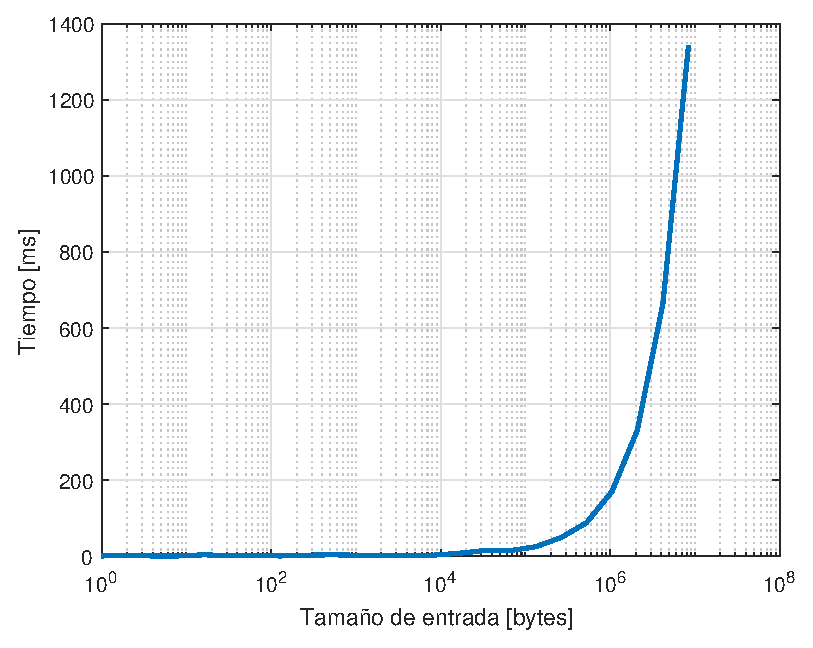
\includegraphics[scale=1]{includes/decodingTimes.eps}
	\caption{Tiempos de ejecución para decodificación.}
	\label{decodeTime}
\end{figure}

\clearpage

%-------------------------------%
%								%
%			Seccion				%
%								%
%-------------------------------%
\section{Herramientas de hardware y software utilizadas}\label{sec_tools}

La computadora utilizada para realizar el desarrollo y las pruebas tiene las siguientes especificaciones:
\begin{itemize}
	\item Procesador: Intel i3-6100.
	\item Memoria: 8GB RAM DDR4.
	\item Almacenamiento: Disco magnético de 200GB de 7200RPM.
\end{itemize}

Los programas se desarrollaron en el sistema operativo Linux Ubuntu, cuyos datos de distribución son
\begin{Verbatim}
	Distributor ID: Ubuntu
	Description: Ubuntu 16.04.2 LTS
	Release: 16.04
	Codename: xenial
\end{Verbatim}

Además, se utilizaron las siguientes herramientas:
\begin{itemize}
	\item \underline{Compilador del proyecto}: GNU gcc (Ubuntu 5.4.0-6ubuntu1~16.04.4) 5.4.0 20160609 \cite{tool_gcc}.
	\item \underline{Control del proceso de compilación}: GNU Make 4.1 \cite{tool_gnuMake}.
	\item \underline{Compilador del presente informe}: Latex pdfTeX 3.14159265-2.6-1.40.16 (TeX Live 2015/Debian) \cite{tool_latex}.
    \item \underline{Edición de código fuente}: VIM - Vi IMproved 7.4 (2013 Aug 10, compiled Nov 24 2016 16:44:48) y Atom 1.15.0 \cite{tool_vim} \cite{tool_atom}.
	\item \underline{Depuración del programa}: gdb \cite{tool_gdb}.
\end{itemize}

%-------------------------------%
%								%
%			Seccion				%
%								%
%-------------------------------%
\section{Conclusiones}

Se creó un programa en lenguaje C que permite codificar y decodificar información en formato base 64, cumpliendo con las especificaciones del enunciado del trabajo. Se describió el flujo del programa y las funciones y estructuras más importantes del mismo, junto con el manejo de errores. Además, se describió el modo de compilación del programa utilizando las herramientas \texttt{gcc} y \texttt{make}.

Por otro lado, se crearon casos de prueba de caja negra para verificar el correcto funcionamiento del programa. Las mismas cubren tests de validación de opciones del programa ingresando combinaciones de opciones válidas e inválidas para determinar si este es capaz de detectar errores. Además, se crearon pruebas de codificación y decodificación de archivos, tamaños máximos de líneas, y tiempos de ejecución.

De esta forma se deja lista la infraestructura básica para los siguientes proyectos donde se trabajará con la arquitectura MIPS32 y el consecuente análisis y desarrollo de código assembly MIPS32.
%-------------------------------%
%								%
%			Seccion				%
%								%
%-------------------------------%
\clearpage
\begin{thebibliography}{10}
	%	\bibitem{book_CompArch} Hennessy, J. L. - Patterson, D. A. - \emph{Computer Architecture: A Quantitative Approach} - 3\textsuperscript{rd} edition - Morgan Kaufmann - 2002.
	%	\bibitem{book_CompOrg} Patterson, D. A. - Hennessy, J. L. - \emph{Computer Organization and Design: The Hardware/Software Interface} - 3\textsuperscript{rd} edition - Morgan Kaufmann - 2004.
	\bibitem{book_Cprogr} Kernighan, B. W. - Ritchie, D. M. - \emph{C Programming Language} - 2\textsuperscript{nd} edition - Prentice Hall - 1988.
	\bibitem{book_patton} Patton, R. - \emph{Software Testing} - 2\textsuperscript{nd} edition - Sams Indianapolis, IN, USA 2005.
	\bibitem{apuntes} \emph{Apuntes del curso 66.20 Organización de Computadoras} - Cátedra Hamkalo - Facultad de Ingeniería de la Universidad de Buenos Aires.
	\bibitem{rfc2045} \emph{RFC 2045} - \hyperlink{make}{https://tools.ietf.org/html/rfc2045\#section-6.8}
	\bibitem{wiki_base64} \emph{Base 64} - \hyperlink{make}{https://en.wikipedia.org/wiki/Base64}
	\bibitem{tool_gnuMake} \emph{GNU Make} - \hyperlink{make}{https://www.gnu.org/software/make/}
	\bibitem{tool_gcc} \emph{GNU Gcc} - \hyperlink{gcc}{https://gcc.gnu.org/}
	\bibitem{tool_latex}
	\href{https://www.latex-project.org/}{\LaTeX - https://www.latex-project.org/}
	\bibitem{tool_vim}
	\href{https://vim.sourceforge.io/}{VIM - https://vim.sourceforge.io/}
	\bibitem{tool_atom}
	\href{https://atom.io/}{Atom - https://atom.io/}
	\bibitem{tool_gdb}
	\href{https://www.gnu.org/software/gdb/}{GNU gdb - https://www.gnu.org/software/gdb/}
\end{thebibliography}
\clearpage

%-----------------------------------%
%									%
%			Seccion:Fuente			%
%									%
%-----------------------------------%
\appendix
\section{Makefile}\label{appendix_makefile}

\subsubsection{makefile}\label{app_makefile}
\lstinputlisting[language=bash, style=StyleC]{src/makefile.make}
\clearpage

\section{Tests}\label{appendix_tests}

\subsubsection{runTests.sh}\label{app_run_tests}
\lstinputlisting[language=bash, style=StyleC]{src/runTests.sh}

\clearpage
\section{Código fuente}\label{appendix_codigo_fuente}

\subsubsection{main.c}\label{app_main}
\lstinputlisting[language=C, style=StyleC]{src/main.c}
\clearpage

\end{document}
